\section{Cross-layer Tool Design}
\label{sec:crossAnalysis}

\textit{TransLayer} is a cross-layer mapping and root cause analyzing tool based on QxDM traces. Even though it requires QxDM to gather information, we claim that such detailed lower layer information empowers us to gain a transparent view across different layers. The primary use case for \textit{TransLayer} is to identify performance issues. We talk about how to collect ground truth data transmission information in IP and RLC layer using QxDM in \S~\ref{subsec:qxdm.tool}. \S~\ref{subsec:cross-layer.mapping} talks about the core algorithm to enable cross-layer mapping between IP and RLC layer. \S~\ref{subsec:uniqueness.analysis} verifies the cross-layer mapping accuracy by showing the unique existence in the whole trace. \S~\ref{subsec:lower.layer.features} lists the major lower features that we utilize to perform root cause analysis.

\subsection{QxDM}
\label{subsec:qxdm.tool}
% Describe what the tool does
QxDM provides the the IP and lower information as input to \textit{TransLayer}. It is a real-time data collection and diagnostic logging tool for measuring mobile-based RF (Radio Frequency) performance~\cite{qxdm_flyer}. It is a Windows based monitoring application. When we perform control experiments and real application measurements, we plug in the device to the desktop or laptop with QxDM software installed. Once the experiments finishes, we filtered out the real-time monitoring information related to IP packets, RLC PDUs, and RRC states in Table~\ref{tab:QxDM.logs}, and dump the results into a log file. The 0x11EB log entry includes IP headers, IP payloads, and its customized header. Since large IP packets will be fragmented into smaller segments, the customer header could indicate the segment index of the whole IP packet. The 0x4132 and 0x4133 unveil the RLC AM configurations, i.e. the polling function timers, the retransmission limit for a single PDU, and etc. The 0x413B, and 0x418B provides RLC PDU header and first byte payload information for both data PDUs and control PDUs (or STATUS PDUs) in both uplink and downlink directions. We wrote a QxDM log parser to aggregate the filtered entries in \textit{TransLayer}, and apply cross-layer mapping to understand the correlation between different layers. We conduct all the experiments on Galaxy S3 with Android OS 4.1.1.

% Table of QxDM entries
\begin{table}[t!]
\begin{tabularx}{0.48\textwidth}{ | c | X | }
	\hline
  	\textbf{QxDM Log ID} & \textbf{Description} \\
  	\hline\hline
  	0x11EB & IP data packets \\
  	\hline
  	0x4132 & WCDMA RLC downlink acknowledge mode configuration \\
  	\hline
  	0x4133 & WCDMA RLC uplink acknowledge mode configuration \\
  	\hline
  	0x413B & WCDMA RLC uplink acknowledge mode PDU \\
  	\hline
  	0x418B & WCDMA Flexible RLC downlink acknowledge mode PDU \\
  	\hline
  	0x4125 & WCDMA RRC states \\
  	\hline
\end{tabularx}
\caption{QxDM log entries used in cross layer analysis}
\label{tab:QxDM.logs}
\end{table}

\subsection{Cross-layer Mapping}
\label{subsec:cross-layer.mapping}
% Describe the mapping algorithm I use for cross-layer analysis
QxDM tool provides fine grained lower layer RLC layer transmission information. If we could correlate the transport layer packets with the RLC layer transmitted PDUs, we will have a transparent view of the link layer behaviors, especially the RLC retransmission. As mentioned in \S~\ref{subsec:partial.logging}, one of the fundamental limitation of QxDM is the partial logging issue. For example, only the header and first byte data payload will be logged for each RLC PDU. It is also possible that a small fraction of RLC PDUs cannot be captured, which lead to a unnecessary sequence number gap. Our mapping algorithm will handle all the limitations we have mentioned.

\begin{figure}[t!]
\centering
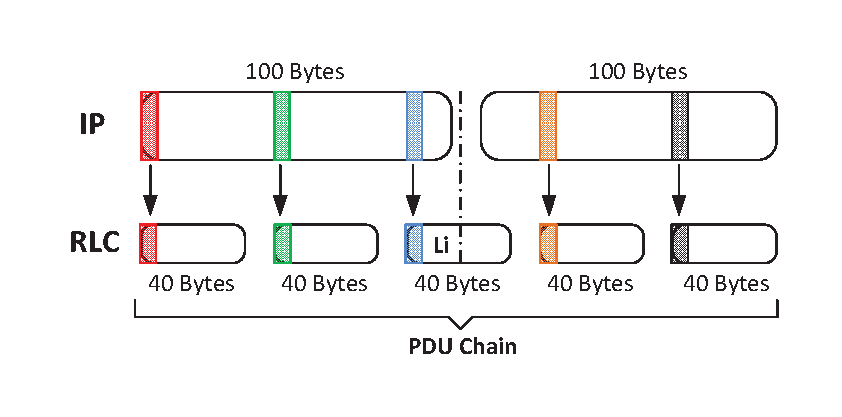
\includegraphics[width=0.5\textwidth]{figs/cross_layer_mapping.eps}
\caption{Cross-layer mapping from IP packets to RLC PDUs chains, where are a sequence of consecutive RLC PDUs. Due to the partial logging, we could only map the limited bytes for every certain length (\textit{long jump mapping}). It is possible that one PDU could concatenate the last part of the first SDU and the first part of the second SDU. Therefore, the five RLC PDU forms a unique RLC PDU chain.}
\label{fig:cross.layer.mapping}
\end{figure}

% The mapping algorithm here
The cross-layer mapping algorithm is the core technique for \textit{TransLayer}. It is essentially a map between the complete IP packets (also known as SDU) and corresponding fragmented RLC payload data bytes (known as PDU). Due to the partial logged information in QxDM, only the first data byte is captured in the log. Thus, we have to skip over the rest of the PDU, and try to match for the first data byte in the next PDU as shown in Figure~\ref{fig:cross.layer.mapping}, which we call the \textit{long jump mapping}. The problem at this point is to determine the end of IP packets while we iterate through the consecutive RLC PDUs. Since each PDU could either contain the payload data dedicated to a single SDU or belongs to two SDUs. If the reminder size of the SDU cannot fulfill the largest size of PDU, then RLC protocol will concatenate the part of the next SDU to fill the rest of space~\cite{spec-3G-RLC} using LI (Length Indicator) in the RLC PDU header. Ultimately, if the accumulative mapped index equals the size of SDU, we claim to find a mapping successfully; otherwise no mapping discovered.

% the corner case of the mapping algorithm
There is a corner case in the mapping algorithm such that the QxDM cannot capture the some of the SDUs. Similar to TCP protocol, the sequence number in RLC PDUs could uniquely distinguish between every PDUs. If there are some missed PDUs, then we cannot map the first byte data for every PDU size. In that case, we could even skip over the missed PDUs and add up multiple of PDU size to hunt for a match. Because of the limitation of the QxDM tool, the \textit{long jump mapping} mechanism cannot fully recover the corner case, especially when the missed PDUs were either the beginning or the end part of the mapped RLC list. We evaluate the improved mapping algorithm by checking the percentage of mapped IP packets in our standard \emph{Browsing Dataset} from \S~\ref{subsec:dataset}, and the average mapping ratio is \textit{99.52\%} for uplink and \textit{88.83\%} for downlink. One reason for a lower the downlink ratio is that the size of PDU is flexible in WCDMA downlink, and the average size is around 17 times greater than that of uplink in our traces. Considering the partial logging information, that actually implies fewer information is available in downlink RLC layer, which leads to a smaller successful mapping ratio.

\subsection{Uniqueness Analysis}
\label{subsec:uniqueness.analysis}
The cross-layer mapping in \S~\ref{subsec:cross-layer.mapping} only claims the existence of cross-layer, but it does not guarantee the mapped RLC PDUs exist once in the trace. We perform uniqueness analysis to prove the uniqueness of the mapped RLC PDUs in the whole trace. One important observation is that RLC SDU concatenation is fairly common as shown in Figure~\ref{fig:cross.layer.mapping}, especially during bulk transmission in transport layer. The concatenation actually introduces some degree of randomness of the partial RLC PDU payload locations. In other word, the cross-layer mapping does not always start from the very first byte in SDU within the same RLC PDU chain. For example, the two SDUs in Figure~\ref{fig:cross.layer.mapping} have different byte placements that mapped to lower layer. 

% Table of uniqueness analysis
\begin{table}[t!]
\begin{tabularx}{0.48\textwidth}{ | c | X | }
	\hline
  	\textbf{Type} & \textbf{Percentage of Unique Mapping (\%)} \\
  	\hline\hline
  	TCP uplink & \multicolumn{1}{|c|}{91.42} \\
  	\hline
  	TCP downlink & \multicolumn{1}{|c|}{88.70} \\
  	\hline
  	UDP uplink & \multicolumn{1}{|c|}{30.86} \\
  	\hline
  	UDP downlink & \multicolumn{1}{|c|}{93.94} \\
  	\hline
\end{tabularx}
\caption{Evaluate the uniqueness of RLC PDU chains in the standard web browsing trace}
\label{tab:uniqueness.analysis}
\end{table}

We analyze the uniqueness of RLC PDU chains, which are essentially a sequence of data bytes in RLC PDU payloads. In Table~\ref{tab:uniqueness.analysis}, after classifying all the PDU chains into guarantee uniqueness and not guarantee uniqueness, we apply cross-layer mapping on our standard \emph{Browsing Dataset} from \S~\ref{subsec:dataset}, and examine the percentage of mapped RLC PDU sequences residing inside an unique RLC PDU chains. We notice that UDP uplink is relative lower than the other three categories. The reason is that the majority of UDP uplink traffic is DNS lookup. The size of the UDP packet is usually less than 70 bytes. Since each uplink RLC PDU is fixed 40 bytes, that implies two PDUs are sufficient to carry a single DNS lookup request. The only information that is useful mapping is the first two bytes, and the 41 and 42 bytes. For a IP packet, the first two bytes is always ``45 00" in IPv4 without exception for DNS lookup. The 41 and 42 byte are actually the first two bytes of the request URLs, which are most likely to be the first two bytes of string ``www". To make it worse, the mapped RLC PDUs are usually stand alone without help from SDU concatenation. Therefore, UDP uplink is much worse than the other three categories.

\subsection{Lower Layer Features}
\label{subsec:lower.layer.features}

\subsubsection{RLC Retransmission}
As mentioned in \S~\ref{subsec:background.rlc}, RLC protocol is implemented with ARQ mechanism. Once the sender received the STATUS PDU from the receiver, any unreceived RLC PDU will be preempted to be retransmitted from the retransmission buffer~\cite{spec-3G-RLC}. In Figure~\ref{fig:rlc.protocol}, the payload of STATUS PDU is a sequence of number pairs. The first number is the starting index of unreceived RLC PDU sequence number, and the second number indicates the length of consecutive unreceived RLC PDUs from that starting sequence number. In this case, the second and the third PDU are not received by the receiver. 

Due to the header size limitation of RLC PDU, sequence number is assigned with period of 4096 in both uplink and downlink (rare exceptional cases are possible). Because of the partial logging information, STATUS PDU payload is not complete, so we cannot directly allocate the retransmitted RLC PDUs from those control message. Instead, \textit{TransLayer} follows the periodical sequence number reuse rule to capture the smaller period for sequence number reuse as a sign of RLC PDU retransmission. \textit{TransLayer} labels the retransmitted RLC PDUs as a pre-process so that we could determine the number of retransmitted RLC PDU within a mapped RLC PDU chain as RLC retransmission count. The RLC retransmission ratio is defined as RLC retransmission count divided by the total number of PDU in a RLC PDU chain.

\subsubsection{First-hop Latency}
The first-hop latency is defined as combination of transmission delay of all the RLC PDUs that belongs to the same IP packet, and the OTA (over the air) RTT in Figure~\ref{fig:cell.topology}. \textit{TransLayer} considers the two latency values separately. Transmission delay is the time difference between the first transmitted PDUs and the last one. We would also want to normalize the transmission delay by dividing the number of mapped RLC PDUs. OTA RTT is essentially the one-way delay from the device to Node B or eNB. As mentioned in \S~\ref{subsec:loose.rlc.rtt.estimation}, it is not feasible to accurately calculate the specific RTT for every RLC PDU (we can for those header enables the polling request bit). \textit{TransLayer} uses the nearest available RTT as an approximation for OTA delay.

\subsubsection{Power}
There are two important power feature that could infer the traffic load in the cellular network: UE received signal strength and SNR (Signal-to-Noise Ratio)~\cite{loadsense}. Signal strength is the received signal power from Node B or eNB, which could be used a relative value to indicate the channel quality. It is usually be referred as RSCP (Received Signal Code Power) in WCDMA and as RSRP (Reference Signal Received Power) in LTE. SNR is a indicator value that combines the pilot power with the inference from other subcarriors. In WCDMA, it is called ECIO (Energy / Interference) in WCDMA and RSRQ (Reference Signal Received Quality) in LTE. \textit{TransLayer} collects all those context information and assign to each transport layer packets.




